	\documentclass[a4paper, twocolumn, twoside, 11pt]{article}
	\usepackage{workshoppreamble}
	%\raggedbottom
	
%	-	-	-	-	-	-	-	-	-	-	-	-	-	-	-	-	-	-	-	-

\begin{document}

	%Title
	\author{Manchester Raspberry Jam}
	\title{Workshop 12a: Introduction to Raspberry Pi and PIXEL}
	\date{}
	\maketitle
	
%	PDF available at \url{bit.ly/mcrraspjam}
	
	%Table of Contents
	\setcounter{tocdepth}{1}
	\tableofcontents
	
	%Contents
	\setcounter{section}{-1}
	\section{Introduction}
		We usually have a full set of notes for our main workshop. This time, we'll be skimming over a lot of programs that have been better covered by other people.
		
		So following on from the NOOBS setup guide in section \ref{sec:NOOBS}, section \ref{sec:Resources} will be a compilation of various sources of Raspberry Pi tutorials and guides.
		
		These booklets were created using {\fontfamily{rfdefault}\selectfont \LaTeX}, an advanced typesetting system for several sorts of books, reports and letters.
		
		To allow modification and redistribution of these booklets, they are distributed under the CC BY-SA 4.0 License.
	
	\section{Installing NOOBS}
\label{sec:NOOBS}

	On most Raspberry Pis, we usually run an operating system called Raspbian, which is a variant of the GNU/Linux operating system.
	
%	\begin{aside}
%		Because the ARM processor in the Raspberry Pi is similar those found in billions of smartphones around the world, there are lots of other operating systems to choose from, such as other Linux distributions like Ubuntu or Arch, mobile OS's such as Android, and even a variant of Windows 10.
%	\end{aside}
	
	Raspbian can be quite tricky to install on an SD card, so a piece of software called NOOBS is provided to do most of the work for us.
	
	Many Raspberry Pi retailers sell SD cards with NOOBS pre-installed, but if you have a spare 8GB or larger MicroSD card, installing it yourself is straightforward.

	\subsection{Download and Install}
	
	The following instructions are for Windows 10, but should be fairly similar to most operating systems, including other versions of Windows, and MacOS.
		
	
		\begin{enumerate}[nosep]
			\item \textbf{Format your MicroSD card as a FAT file system.}
			
			On windows, right click on the SD card in the file explorer, and click `Format...'.	Most settings can be left as normal, ensure the file systems is set to `FAT32', then press Start.
			
			\begin{center}
				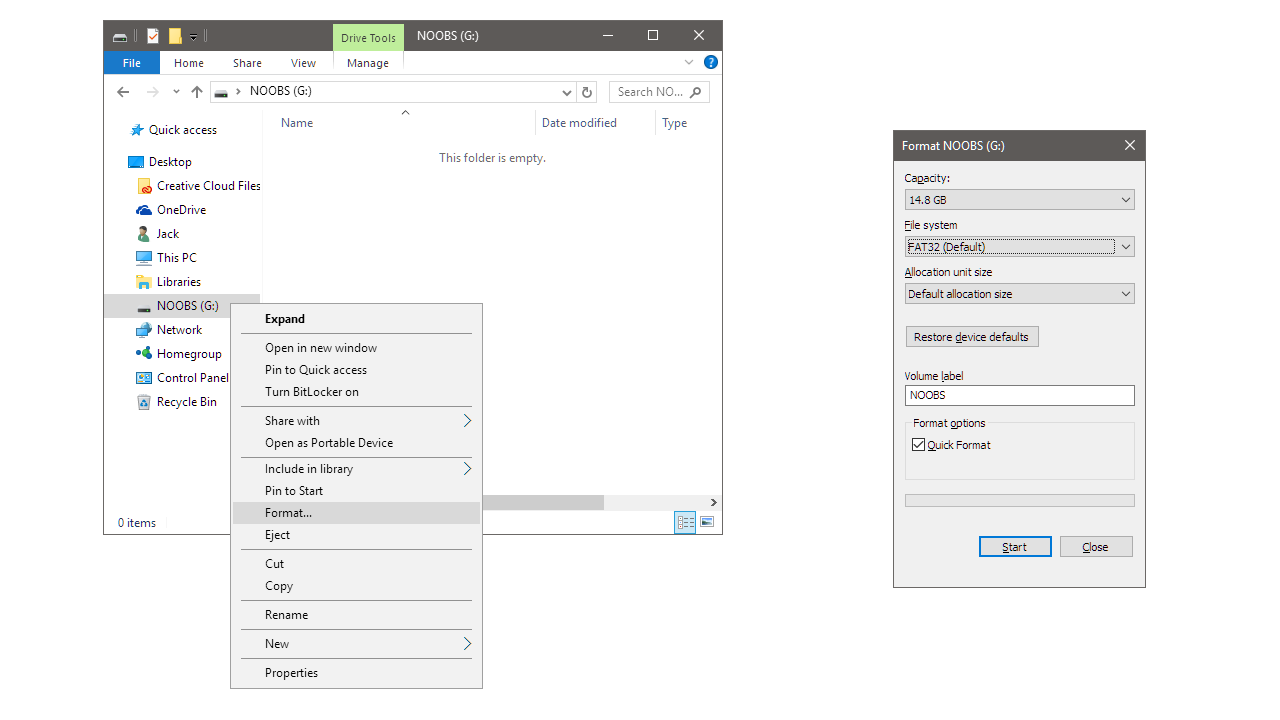
\includegraphics[width=1\linewidth]{sections/1_NOOBS/noobs2}
			\end{center}
			
			\item \textbf{Download the latest version of NOOBS} from \url{https://www.raspberrypi.org/downloads/}
			
			Click the `Download ZIP' button of NOOBS on the following page.
			
			\begin{center}
				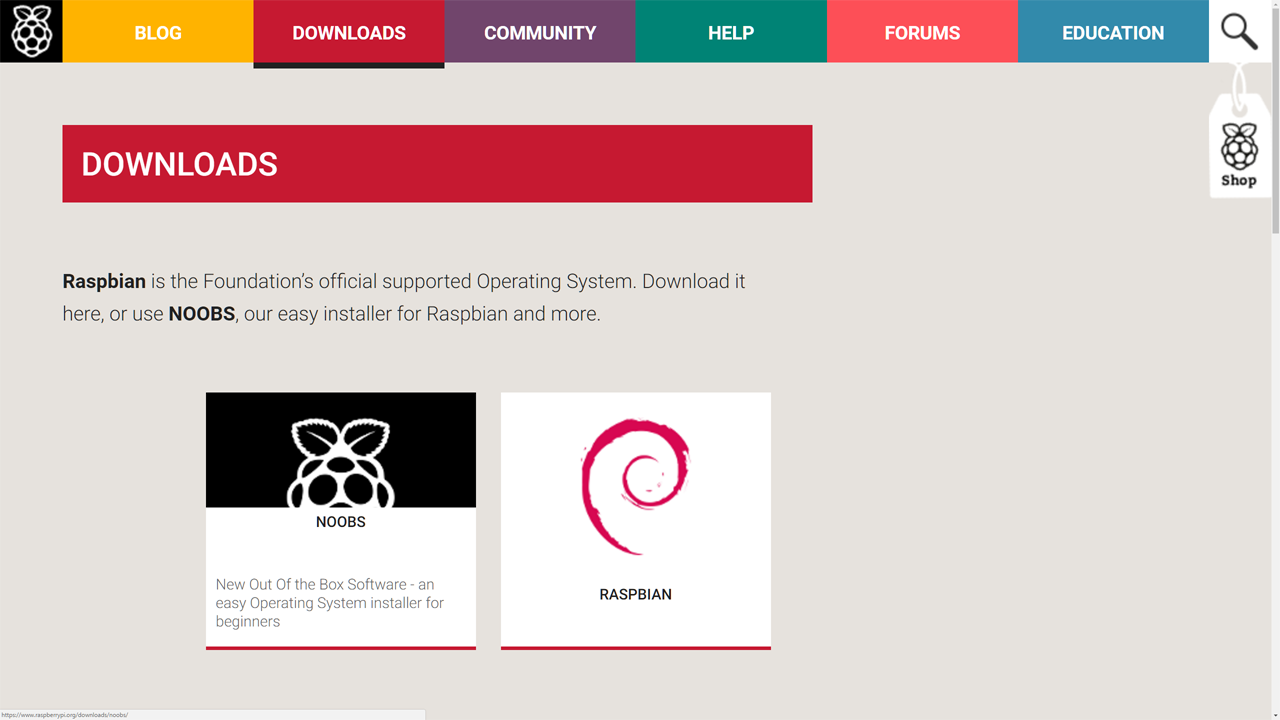
\includegraphics[width=0.8\linewidth]{sections/1_NOOBS/noobs1}
			\end{center}
			
			\item \textbf{Extract the downloaded NOOBS ZIP file onto the SD card}.
			
			On windows, you can right click and `Extract All...' to the drive letter of your SD card e.g. `G:\textbackslash'.
			
			\begin{center}
				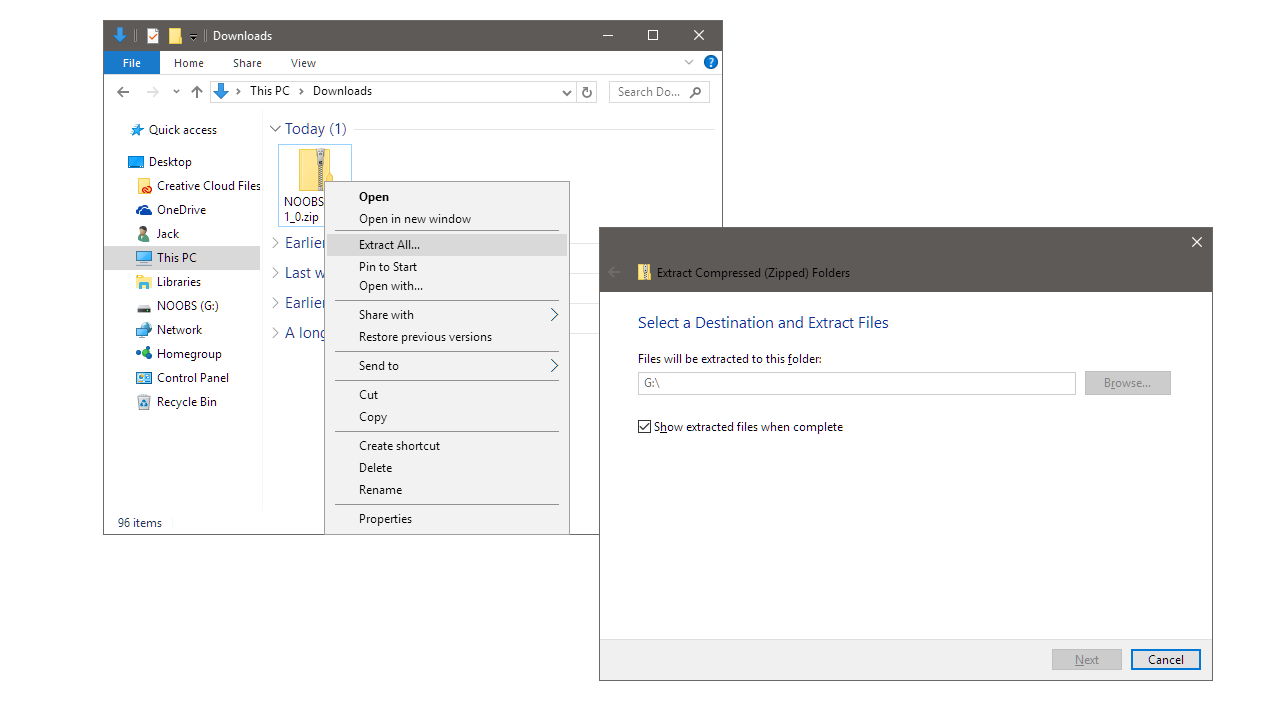
\includegraphics[width=1\linewidth]{sections/1_NOOBS/noobs3}
			\end{center}
		\end{enumerate}
		
		Ensure the files are extracted to the top level of the SD card, and not inside a subfolder.
		
		\subsection{Booting and Installing Raspbian}
		
		Once you have a NOOBs card set up, you can boot your Pi with it. You should see a screen like the following.
		
		\begin{center}
			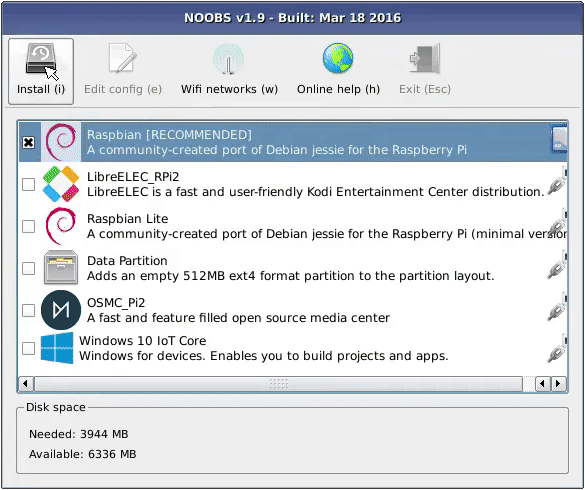
\includegraphics[width=0.8\linewidth]{sections/1_NOOBS/noobs5}
		\end{center}
		
		Select Raspbian (which is the only option when offline) and click install. Follow through any prompts until you reach a loading screen.
		
		The rest of the process is automatic -- and very slow -- so now is the time to find something to do for the next 20 minutes!
		
		
	

	\section{Tutorial Resources}
\label{sec:Resources}

	Below are some top sources guides and tutorials for the Raspberry Pi 
	
	\subsection{Raspberry Pi Tutorials}
	
		\subsubsection*{Raspberry Pi Resources}
	
			\url{https://www.raspberrypi.org/resources/}
			\begin{center}
				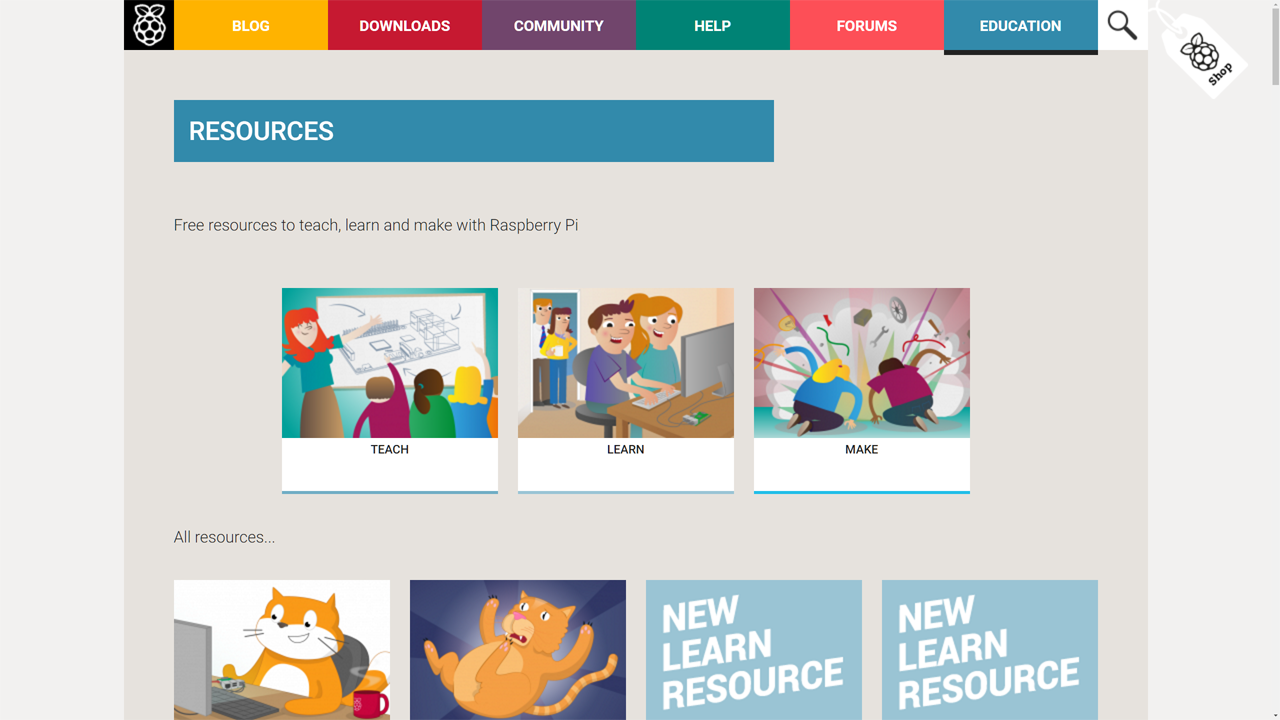
\includegraphics[width=0.5\linewidth]{sections/2_Resources/raspberrypiorg}
			\end{center}

	
			The official Raspberry Pi website should be your first stop, it's chock full of introduction tutorials and project ideas for most of the software we've covered today.
	
		\subsubsection*{The MagPi Magazine}
	
			\url{https://www.raspberrypi.org/magpi/}
			\begin{center}
				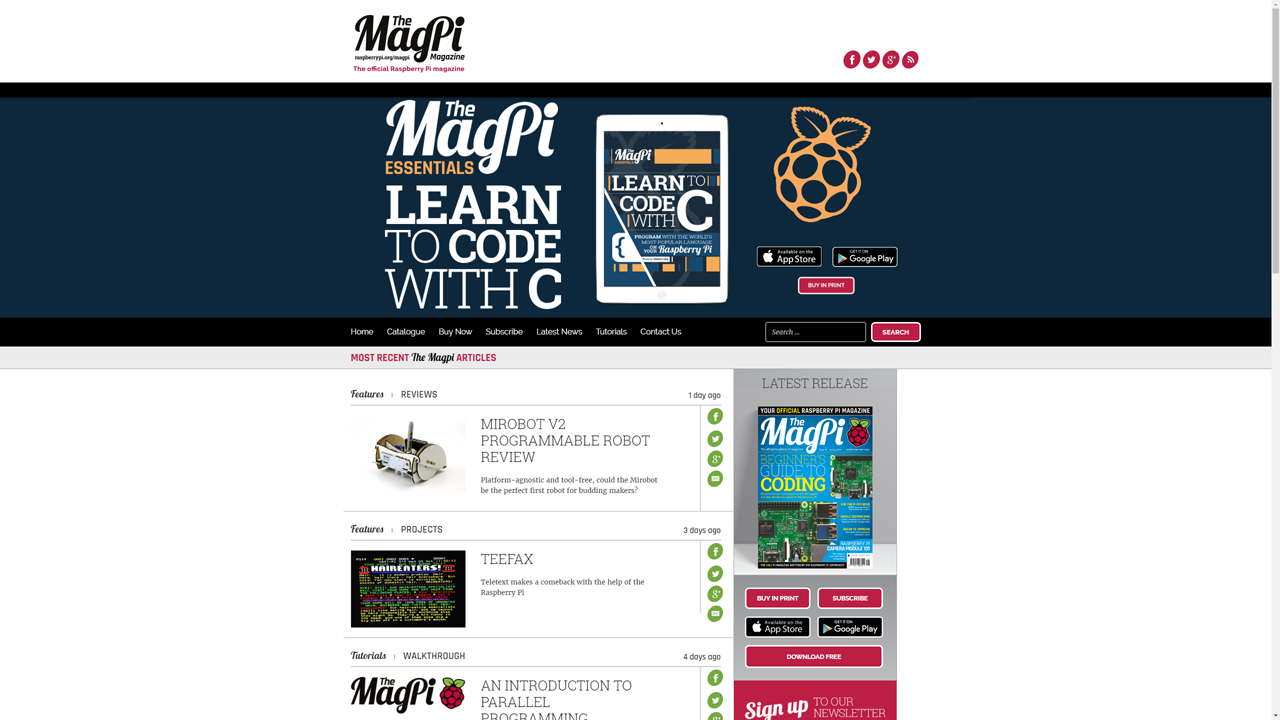
\includegraphics[width=0.5\linewidth]{sections/2_Resources/magpi}
			\end{center}		
				
			The MagPi started as a community run print magazine for the Raspberry Pi, and has now become the official magazine of the Raspberry Pi.
			
			Available in print (can be found in many supermarkets), or as a free download, each one is filled with articles, features and tutorials, all for the Raspberry Pi.
			
		\subsubsection*{The Raspberry Pi Guy}
			
			\url{http://www.theraspberrypiguy.com/tutorials/}
			\begin{center}
				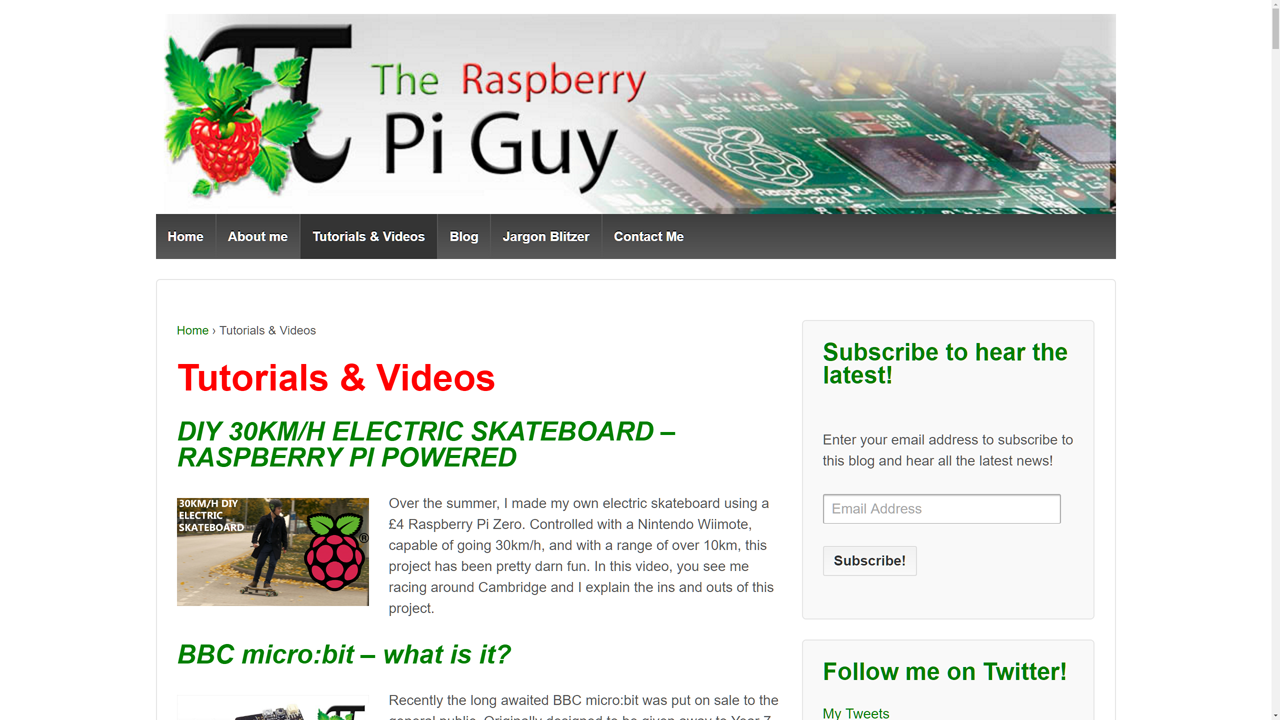
\includegraphics[width=0.5\linewidth]{sections/2_Resources/piguy}
			\end{center}	
			
			Matt was one of the first people to start producing regular video content for the Raspberry Pi, he was only 12 when the Pi was first released!
			
			Every few months, he produces a new video tutorial, showing off cool projects and uses for the Raspberry Pi, covering things as wide as Steam game streaming, robotics, or even building an electric skateboard.
		
	\subsection{Programming Language Tutorials}
	
		Ready to stretch your legs and try another programming language? Here are some quality tutorials for learning some new languages.
		
		\url{https://www.codecademy.com/learn/learn-java}
		
		Java has big long lines of code which look scarier than they are, but it's a great second language to learn, and a great introduction to object orientated programming.
		
		\textit{We'll have more here on the online version of these notes soon. In the meantime, why not ask us at today's Pi Clinic? We'll be able to find and recommend books and online tutorials for anything you might like to learn.}
	
		
	
\iffalse
	
		Ready to stretch your legs and try another programming language? Here are some quality tutorials for learning some new languages.
		
		\subsubsection*{If you want to try something else:}
		
			\url{https://www.codecademy.com/learn/learn-java}
			
			Java has big long lines of code which look scarier than they are, but it's a great second language to learn, and a great introduction to object orientated programming.
		
		\subsubsection*{If you're feeling brave:}
		
			\url{http://www.learn-c.org/}
			
			C is 45 years old. It's one of the oldest programming languages still in use, but with good reason.
			
			It's a familiar language syntax to things like Java, and pointers provide a challenge that's difficult to grasp at first, but very rewarding.
	
		\subsubsection*{If you're feeling foolhardy:}
		
			\url{http://www.learncpp.com/}
			
			Linus Torvalds and a few others may disagree, but C++ aimed to build on the foundations of C.
			
			This language will provide a challenge, but it's one of the most widely used programming languages there is. You can even use it to jump off into things like graphics rendering (\url{https://learnopengl.com/})
		
		\subsubsection*{If you're just feeling silly, now:}
		
			\url{https://www.codecademy.com/learn/php}
			
			A scary looking syntax, but PHP forms the majority of server-side code on the modern web. If you're already planning far ahead for a move into web development, you'll want to learn some PHP.
		
		\subsubsection*{If you want to build web apps:}
		
			\url{https://www.codecademy.com/learn/learn-javascript}
			
			If you want your webpages to do more than just display text, Javascript is the most common programming language used in the web today.
			
			Once you've learnt the basics, you'll 
\fi	

\end{document}